% !Mode:: "TeX:UTF-8"
\documentclass[12pt,a4paper]{article}

%%%%%%%%------------------------------------------------------------------------
%%%% 日常所用宏包

%% 控制页边距
% 如果是beamer文档类, 则不用geometry
\makeatletter
\@ifclassloaded{beamer}{}{\usepackage[top=2.5cm, bottom=2.5cm, left=2.5cm, right=2.5cm]{geometry}}
\makeatother

%% 控制项目列表
\usepackage{enumerate}

%% 多栏显示
\usepackage{multicol}

%% 算法环境
\usepackage{algorithm}  
\usepackage{algorithmic} 
\usepackage{float} 

%% 网址引用
\usepackage{url}

%% 控制矩阵行距
\renewcommand\arraystretch{1.4}

%% hyperref宏包,生成可定位点击的超链接,并且会生成pdf书签
\makeatletter
\@ifclassloaded{beamer}{
\usepackage{hyperref}
\usepackage{ragged2e} % 对齐
}{
\usepackage[%
    pdfstartview=FitH,%
    CJKbookmarks=true,%
    bookmarks=true,%
    bookmarksnumbered=true,%
    bookmarksopen=true,%
    colorlinks=true,%
    citecolor=blue,%
    linkcolor=blue,%
    anchorcolor=green,%
    urlcolor=blue%
]{hyperref}
}
\makeatother



\makeatletter % 如果是 beamer 不需要下面两个包
\@ifclassloaded{beamer}{
\mode<presentation>
{
} 
}{
%% 控制标题
\usepackage{titlesec}
%% 控制目录
\usepackage{titletoc}
}
\makeatother

%% 控制表格样式
\usepackage{booktabs}

%% 控制字体大小
\usepackage{type1cm}

%% 首行缩进,用\noindent取消某段缩进
\usepackage{indentfirst}

%% 支持彩色文本、底色、文本框等
\usepackage{color,xcolor}

%% AMS LaTeX宏包: http://zzg34b.w3.c361.com/package/maths.htm#amssymb
\usepackage{amsmath,amssymb}
%% 多个图形并排
\usepackage{subfig}
%%%% 基本插图方法
%% 图形宏包
\usepackage{graphicx}
\newcommand{\red}[1]{\textcolor{red}{#1}}
\newcommand{\blue}[1]{\structure{#1}}
\newcommand{\brown}[1]{\textcolor{brown}{#1}}
\newcommand{\green}[1]{\textcolor{green}{#1}}


%%%% 基本插图方法结束

%%%% pgf/tikz绘图宏包设置
\usepackage{pgf,tikz}
\usetikzlibrary{shapes,automata,snakes,backgrounds,arrows}
\usetikzlibrary{mindmap}
%% 可以直接在latex文档中使用graphviz/dot语言,
%% 也可以用dot2tex工具将dot文件转换成tex文件再include进来
%% \usepackage[shell,pgf,outputdir={docgraphs/}]{dot2texi}
%%%% pgf/tikz设置结束


\makeatletter % 如果是 beamer 不需要下面两个包
\@ifclassloaded{beamer}{

}{
%%%% fancyhdr设置页眉页脚
%% 页眉页脚宏包
\usepackage{fancyhdr}
%% 页眉页脚风格
\pagestyle{plain}
}

%% 有时会出现\headheight too small的warning
\setlength{\headheight}{15pt}

%% 清空当前页眉页脚的默认设置
%\fancyhf{}
%%%% fancyhdr设置结束


\makeatletter % 对 beamer 要重新设置
\@ifclassloaded{beamer}{

}{
%%%% 设置listings宏包用来粘贴源代码
%% 方便粘贴源代码,部分代码高亮功能
\usepackage{listings}

%% 设置listings宏包的一些全局样式
%% 参考http://hi.baidu.com/shawpinlee/blog/item/9ec431cbae28e41cbe09e6e4.html
\lstset{
showstringspaces=false,              %% 设定是否显示代码之间的空格符号
numbers=left,                        %% 在左边显示行号
numberstyle=\tiny,                   %% 设定行号字体的大小
basicstyle=\footnotesize,                    %% 设定字体大小\tiny, \small, \Large等等
keywordstyle=\color{blue!70}, commentstyle=\color{red!50!green!50!blue!50},
                                     %% 关键字高亮
frame=shadowbox,                     %% 给代码加框
rulesepcolor=\color{red!20!green!20!blue!20},
escapechar=`,                        %% 中文逃逸字符,用于中英混排
xleftmargin=2em,xrightmargin=2em, aboveskip=1em,
breaklines,                          %% 这条命令可以让LaTeX自动将长的代码行换行排版
extendedchars=false                  %% 这一条命令可以解决代码跨页时,章节标题,页眉等汉字不显示的问题
}}
\makeatother
%%%% listings宏包设置结束


%%%% 附录设置
\makeatletter % 对 beamer 要重新设置
\@ifclassloaded{beamer}{

}{
\usepackage[title,titletoc,header]{appendix}
}
\makeatother
%%%% 附录设置结束


%%%% 日常宏包设置结束
%%%%%%%%------------------------------------------------------------------------


%%%%%%%%------------------------------------------------------------------------
%%%% 英文字体设置结束
%% 这里可以加入自己的英文字体设置
%%%%%%%%------------------------------------------------------------------------

%%%%%%%%------------------------------------------------------------------------
%%%% 设置常用字体字号,与MS Word相对应

%% 一号, 1.4倍行距
\newcommand{\yihao}{\fontsize{26pt}{36pt}\selectfont}
%% 二号, 1.25倍行距
\newcommand{\erhao}{\fontsize{22pt}{28pt}\selectfont}
%% 小二, 单倍行距
\newcommand{\xiaoer}{\fontsize{18pt}{18pt}\selectfont}
%% 三号, 1.5倍行距
\newcommand{\sanhao}{\fontsize{16pt}{24pt}\selectfont}
%% 小三, 1.5倍行距
\newcommand{\xiaosan}{\fontsize{15pt}{22pt}\selectfont}
%% 四号, 1.5倍行距
\newcommand{\sihao}{\fontsize{14pt}{21pt}\selectfont}
%% 半四, 1.5倍行距
\newcommand{\bansi}{\fontsize{13pt}{19.5pt}\selectfont}
%% 小四, 1.5倍行距
\newcommand{\xiaosi}{\fontsize{12pt}{18pt}\selectfont}
%% 大五, 单倍行距
\newcommand{\dawu}{\fontsize{11pt}{11pt}\selectfont}
%% 五号, 单倍行距
\newcommand{\wuhao}{\fontsize{10.5pt}{10.5pt}\selectfont}
%%%%%%%%------------------------------------------------------------------------


%% 设定段间距
\setlength{\parskip}{0.5\baselineskip}

%% 设定行距
\linespread{1}


%% 设定正文字体大小
% \renewcommand{\normalsize}{\sihao}

%制作水印
\RequirePackage{draftcopy}
\draftcopyName{XTUMESH}{100}
\draftcopySetGrey{0.90}
\draftcopyPageTransform{40 rotate}
\draftcopyPageX{350}
\draftcopyPageY{80}

%%%% 个性设置结束
%%%%%%%%------------------------------------------------------------------------


%%%%%%%%------------------------------------------------------------------------
%%%% bibtex设置

%% 设定参考文献显示风格
% 下面是几种常见的样式
% * plain: 按字母的顺序排列,比较次序为作者、年度和标题
% * unsrt: 样式同plain,只是按照引用的先后排序
% * alpha: 用作者名首字母+年份后两位作标号,以字母顺序排序
% * abbrv: 类似plain,将月份全拼改为缩写,更显紧凑
% * apalike: 美国心理学学会期刊样式, 引用样式 [Tailper and Zang, 2006]

\makeatletter
\@ifclassloaded{beamer}{
\bibliographystyle{apalike}
}{
\bibliographystyle{unsrt}
}
\makeatother


%%%% bibtex设置结束
%%%%%%%%------------------------------------------------------------------------

%%%%%%%%------------------------------------------------------------------------
%%%% xeCJK相关宏包

\usepackage{xltxtra,fontspec,xunicode}
\usepackage[slantfont, boldfont]{xeCJK} 

%% 针对中文进行断行
\XeTeXlinebreaklocale "zh"             

%% 给予TeX断行一定自由度
\XeTeXlinebreakskip = 0pt plus 1pt minus 0.1pt

%%%% xeCJK设置结束                                       
%%%%%%%%------------------------------------------------------------------------

%%%%%%%%------------------------------------------------------------------------
%%%% xeCJK字体设置

%% 设置中文标点样式,支持quanjiao、banjiao、kaiming等多种方式
\punctstyle{kaiming}                                        
                                                     
%% 设置缺省中文字体
\setCJKmainfont[BoldFont={Adobe Heiti Std}, ItalicFont={Adobe Kaiti Std}]{Adobe Song Std}   
%% 设置中文无衬线字体
\setCJKsansfont[BoldFont={Adobe Heiti Std}]{Adobe Kaiti Std}  
%% 设置等宽字体
\setCJKmonofont{Adobe Heiti Std}                            

%% 英文衬线字体
\setmainfont{DejaVu Serif}                                  
%% 英文等宽字体
\setmonofont{DejaVu Sans Mono}                              
%% 英文无衬线字体
\setsansfont{DejaVu Sans}                                   

%% 定义新字体
\setCJKfamilyfont{song}{Adobe Song Std}                     
\setCJKfamilyfont{kai}{Adobe Kaiti Std}
\setCJKfamilyfont{hei}{Adobe Heiti Std}
\setCJKfamilyfont{fangsong}{Adobe Fangsong Std}
\setCJKfamilyfont{lisu}{LiSu}
\setCJKfamilyfont{youyuan}{YouYuan}

%% 自定义宋体
\newcommand{\song}{\CJKfamily{song}}                       
%% 自定义楷体
\newcommand{\kai}{\CJKfamily{kai}}                         
%% 自定义黑体
\newcommand{\hei}{\CJKfamily{hei}}                         
%% 自定义仿宋体
\newcommand{\fangsong}{\CJKfamily{fangsong}}               
%% 自定义隶书
\newcommand{\lisu}{\CJKfamily{lisu}}                       
%% 自定义幼圆
\newcommand{\youyuan}{\CJKfamily{youyuan}}                 

%%%% xeCJK字体设置结束
%%%%%%%%------------------------------------------------------------------------

%%%%%%%%------------------------------------------------------------------------
%%%% 一些关于中文文档的重定义
\newcommand{\chntoday}{\number\year\,年\,\number\month\,月\,\number\day\,日}
%% 数学公式定理的重定义

%% 中文破折号,据说来自清华模板
\newcommand{\pozhehao}{\kern0.3ex\rule[0.8ex]{2em}{0.1ex}\kern0.3ex}

\newtheorem{example}{例}                                   
\newtheorem{theorem}{定理}[section]                         
\newtheorem{definition}{定义}
\newtheorem{axiom}{公理}
\newtheorem{property}{性质}
\newtheorem{proposition}{命题}
\newtheorem{lemma}{引理}
\newtheorem{corollary}{推论}
\newtheorem{remark}{注解}
\newtheorem{condition}{条件}
\newtheorem{conclusion}{结论}
\newtheorem{assumption}{假设}

\makeatletter %
\@ifclassloaded{beamer}{

}{
%% 章节等名称重定义
\renewcommand{\contentsname}{目录}     
\renewcommand{\indexname}{索引}
\renewcommand{\listfigurename}{插图目录}
\renewcommand{\listtablename}{表格目录}
\renewcommand{\appendixname}{附录}
\renewcommand{\appendixpagename}{附录}
\renewcommand{\appendixtocname}{附录}
%% 设置chapter、section与subsection的格式
\titleformat{\chapter}{\centering\huge}{第\thechapter{}章}{1em}{\textbf}
\titleformat{\section}{\centering\sihao}{\thesection}{1em}{\textbf}
\titleformat{\subsection}{\xiaosi}{\thesubsection}{1em}{\textbf}
\titleformat{\subsubsection}{\xiaosi}{\thesubsubsection}{1em}{\textbf}

\@ifclassloaded{book}{

}{
\renewcommand{\abstractname}{摘要}
}
}
\makeatother

\renewcommand{\figurename}{图}
\renewcommand{\tablename}{表}

\makeatletter
\@ifclassloaded{book}{
\renewcommand{\bibname}{参考文献}
}{
\renewcommand{\refname}{参考文献} 
}
\makeatother

\floatname{algorithm}{算法}
\renewcommand{\algorithmicrequire}{\textbf{输入:}}
\renewcommand{\algorithmicensure}{\textbf{输出:}}

%%%% 中文重定义结束
%%%%%%%%------------------------------------------------------------------------


\title{ 程序开发环境及消息传递编程接口 MPI }
\author{}
\date{\chntoday}

\begin{document}
\maketitle
\section{ 程序开发环境 }
\subsection{ vim 编辑器 }
vim是从 vi 发展出来的一个文本编辑器。vim不识别鼠标。首先打开终端,输入vim 文件名,就可以用vim打开一个文件
\begin{figure}[H]
\centering
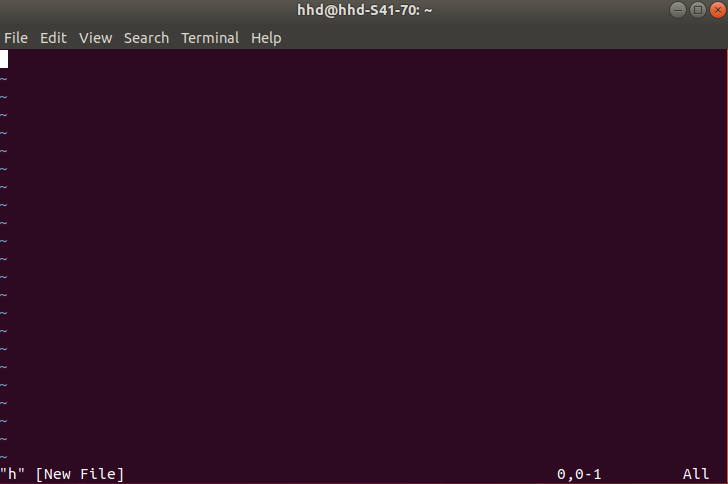
\includegraphics[scale=0.5]{./figures/9.png}
\caption{}
\end{figure}

vim 共分为三种模式,分别是命令模式,输入模式和底线命令模式。

1. 命令模式

以下是常用的几个命令:

i 切换到输入模式,以输入字符。

x 删除当前光标所在处的字符。

: 切换到底线命令模式,以在最底一行输入命令。

2. 输入模式

在命令模式下按下i就进入了输入模式。在输入模式中,可以使用以下按键:

• 移动光标:在命令状态下,移动光标的命令主要有下面一些。

– h 、 j 、 k 、 l 用于上下左右移动光标,如果终端类型配置正确的话也可以用四个箭头键。

– w 和 b 分别将光标向前和向后移动一个单词;

– Ctrl-D 和 Ctrl-U 分别将光标向前和向后移动半个屏幕;

– Ctrl-F 和 Ctrl-B 分别将光标向前和向后移动一个屏幕;

( 翻页 ) ,如果终端类型配置正确的话也可以用 <PgUp> 和<PgDn> 键;

– ) 和 ( 分别将光标向前和向后移动一个句子;

– $\rbrace$ 和 $\lbrace$ 分别将光标向前和向后移动一个段落;

– H,M 和 L 分别将光标移动到屏幕的最上面、中间和最下面一行上;

– nG 将光标移动到第 n 行上,其中 n 是一个整数;

• 删除文本:在命令状态下,x 删除一个字符,dw 删除一个词,d删除当前位置到行尾的所有内容,dd 删除一行;

• 替换文本:在命令状态下按 R 键便进入替换状态,此时新键入的字符会替换光标下原有的字符,按 Esc 键可以回到命令状态;如果在命令状态下按 r 键则会在替换当前光标下的一个字符后自动返回到命令状态;

• 查找和替换文本:在命令状态下按 / 键可以输入一个正则表达式来查找与它匹配的字符串;按 : 键,然后用 s 命令可以进行字符串的替换,命令格式与 sed 的 “s” 命令完全一样。需要注意的是,如同前面指出过的,不同版本的正则表达式在元字符处理上可能会略有不同;

• 拷贝和粘贴文本:当使用删除命令删除了一部分内容以后,被删除的文本被存储在缓冲区中,可以用 p 键将缓冲区中的文本粘贴到当前光标位置的后面;也用 y 命令将指定的文本放到缓冲区中,供后面的粘贴操作使用,y 来源于英文单词 yank,比如 yw 将会拷贝一个词到缓冲区, yy 会拷贝整个一行到缓冲区,
等等;

• 撤销上一次的操作:在命令状态下按 u 键可以撤销上一次的操作。

3. 底线命令模式

在命令模式下按下:(英文冒号)就进入了底线命令模式。在底线命令模式中,基本的命令有(已经省略了冒号):

q 退出程序

w 保存文件

按ESC键可随时退出底线命令模式。
\begin{figure}[H]
\centering
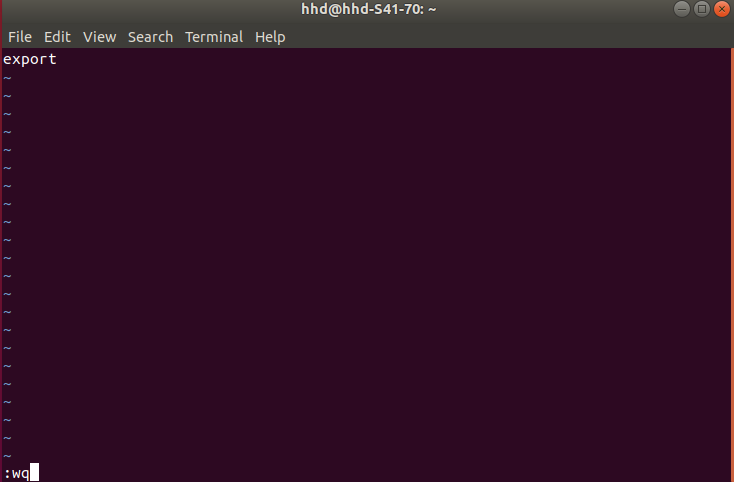
\includegraphics[scale=0.5]{./figures/10.png}
\caption{}
\end{figure}

\subsection{ GCC }
GCC(GNU Compiler Collection,GNU编译器套件),是由 GNU 开发的编程语言编译器。

1. sudo apt-get build-dep gcc--安装gcc编译器

2. 创建hello.c文件
\begin{figure}[H]
\centering
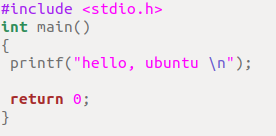
\includegraphics[scale=0.5]{./figures/11.png}
\caption{}
\end{figure}

方法一:

 gcc hello.c--将源文件直接编译成文件名为a.out的可执行文件

 ./a.out--执行a.out可执行文件

方法二:

gcc -o hello hello.c--将hello.c编译输出为一个名称为hello的可执行文件

./hello--执行hello可执行文件

常用编译命令选项:

假设源程序文件名为test.c

1. 无选项编译链接

用法:gcc test.c

作用:将test.c预处理、汇编、编译并链接形成可执行文件。这里未指定输出文件,默认输出为a.out

2. 选项 -o

用法:gcc test.c -o test

作用:将test.c预处理、汇编、编译并链接形成可执行文件test。-o选项用来指定输出文件的文件名

3. 选项 -E

用法:gcc -E test.c -o test.i

作用:将test.c预处理输出test.i文件

4. 选项 -S

用法:gcc -S test.i 

作用:将预处理输出文件test.i汇编成test.s文件

5. 选项 -c

用法:gcc -c test.s

作用:将汇编输出文件test.s编译输出test.o文件

6. 无选项链接
用法:gcc test.o -o test
作用:将编译输出文件test.o链接成最终可执行文件test

7. 选项-O

用法:gcc -O1 test.c -o test

作用:使用编译优化级别1编译程序。级别为1—3,级别越大优化效果越好,但编译时间越长



\subsection{ gdb }
在 Linux 下有很多方便的程序调试工具,其中最基本的调试器是 gdb.gdb 是一个功能非常强大的调试器,下面介绍一下它的简单用法。当需要调试程序时,应该在编译时加上调试选项 “-g” ,它使得可执行文件中包含关于源文件的信息。
首先编译生成可执行文件(test.c)

gcc -g test.c -o test(-g选项告诉gcc在编译程序时加入调试信息)

接下来输入gdb test,就进入了gdb模式
\begin{figure}[H]
\centering
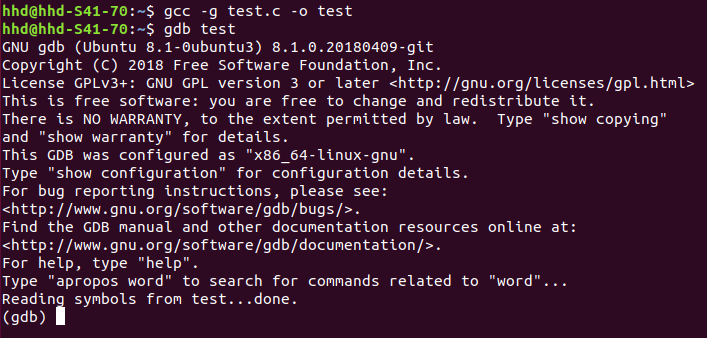
\includegraphics[scale=0.5]{./figures/24.png}
\caption{}
\end{figure}
也可以通过gdb -q test进入gdb模式
\begin{figure}[H]
\centering
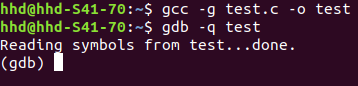
\includegraphics[scale=0.5]{./figures/25.png}
\caption{}
\end{figure}

\begin{figure}[H]
\centering
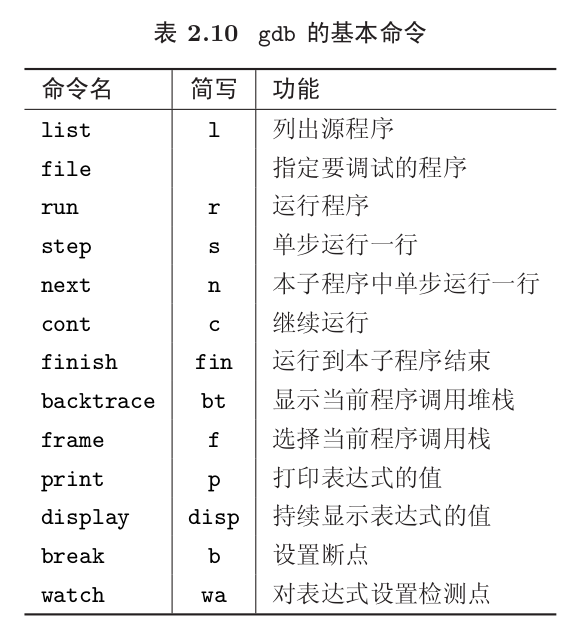
\includegraphics[scale=0.5]{./figures/26.png}
\caption{}
\end{figure}
list默认一次显示10行,list默认参数可以用show listsize来查看。

gdb 还支持字符串查找,search str,从当前行开始,向前查找含str的字符串;

reverse-search str,从当前行开始,向后查找含str的字符串。

输入hell clear,可以达到清屏的效果

看了程序的代码,感觉第6行代码可能有点问题,现在就需要设置一个断点,让程序停在第6行之前。
1说明我设置的这个断点是第一个断点,断点所在内存地址为0x728,它在文件test1.c的第6行。

如果我们想看下设置的断点信息,可以使用info breakpoints命令。
\begin{figure}[H]
\centering
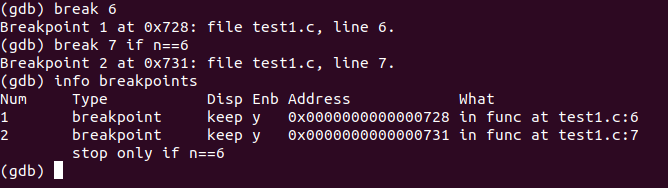
\includegraphics[scale=0.5]{./figures/27.png}
\caption{}
\end{figure}
Num表示断点的编号;Type表示断点的断点的类型,第二个断点类型还加上了条件;Disp表示中断点在执行一次之后是否失去作用,dis为是,keep为不是;Enb表示当前中断点是否有效,y为是,n为否;Address表示中断点所处的内存地址;What指出断点所处的位置。

如果不需要程序在该断点暂停时,有两种方法,一种是使该断点失效,一种是直接删除该断点。
\begin{figure}[H]
\centering
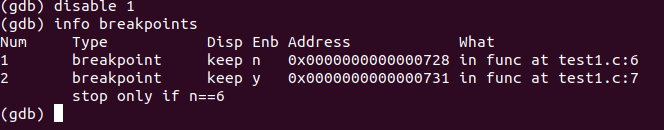
\includegraphics[scale=0.5]{./figures/28.png}
\caption{}
\end{figure}
可以看到,第一个断点的Enb变为n了,表示该断点已经无效了。

直接删除该断点,可以使用clear命令和delete命令。
\begin{figure}[H]
\centering
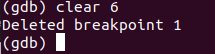
\includegraphics[scale=0.5]{./figures/29.png}
\caption{}
\end{figure}
clear命令后面的参数为设置断点的行号,这里是删除第1个断点

(gdb) delete

删除所有断点吗? (y or n) 

quit--退出gdb调试

kill命令,结束当前程序的调试,不会退出gdb

\subsection{ Fortran 程序的开发 }
新建工作目录文件夹,如“HELLO”,在文件夹中创建“.f”文件,如“HELLO.f”,在“HELLO.f”里面写入
\begin{figure}[H]
\centering
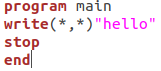
\includegraphics[scale=0.5]{./figures/30.png}
\caption{}
\end{figure}
注意每一行前面都要嵌入一个Tab键,保存文件,在当前目录下打开终端,输入命令:gfortran HELLO.f ,就会产生“a.out”的可执行文件。输入命令:./a.out执行该文件
\begin{figure}[H]
\centering
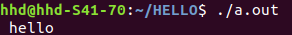
\includegraphics[scale=0.5]{./figures/31.png}
\caption{}
\end{figure}

使用工具nm 查看可执行文件中的内容,会得到下面的信息
\begin{figure}[H]
\centering
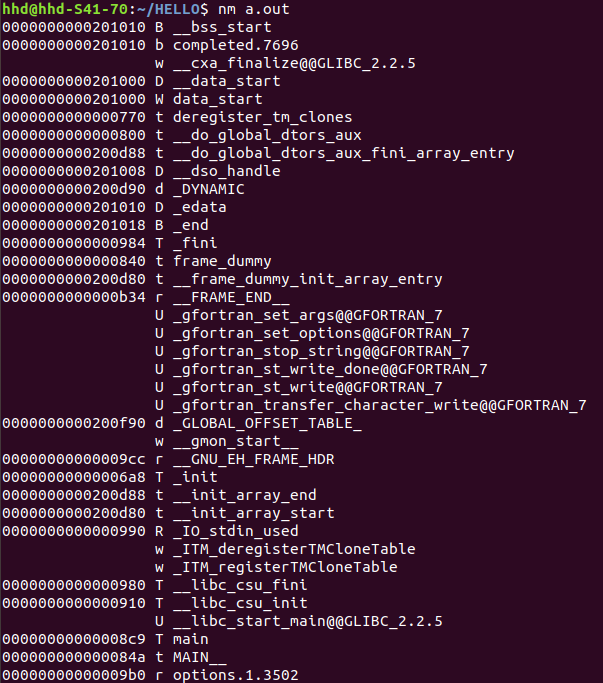
\includegraphics[scale=0.5]{./figures/32.png}
\caption{}
\end{figure}

\subsection{ make }
make,指一条计算机指令,该指令是读入一个名为makefile的文件,然后执行这个文件中指定的指令。

Makefile 是一个包含一系列规则的文本文件。每个规则定义一个目标所依赖的对象和处理命令。每个规则由两部分组成。第一部分是依赖关系,第二部分是处理命令,其中第二部分可以省略。当更新一个指定的目标时, make 会先检查并且在必要时更新它所依赖的每个对象,然后将目标文件的修改时间依次与每个依赖对象文件的修改时间进行比较,如果任何一个依赖对象比目标新,则执行处理命令来对目标进行更新。由于检查依赖关系时,所依赖的对象会先被检查,而这些对象可能又依赖于其他对象,从而检查过程是递归进行的,整个依赖关系形成一个复杂的树形结构。

通过makefile文件中描述源程序之间的依赖关系进行自动编译;makefile文件是按照规定格式编写,需说明如何编译各个源文件并连接生成可执行文件,并要求定义源文件之间的依赖关系; 

基于源文件的改动,make可以自动知道那些文件需要更新;它也会自动决定文件更新的适当顺序,以避免要更新的文件依赖于另一个同样需要更新的文件。因此,在你修改了程序的源代码并且执行make后,你不必重新完全编译你的所有文件,只需要重新编译那些直接或间接受到影响的文件就好了。

\subsection{ Doxygen }
Doxygen 的主页在http://www.stack.nl/~dimitri/doxygen它包含在许多 Linux 发行版中。使用该软件生成文档,需要完成的
事情包括:在程序中按规定的格式写注释、准备一个配置文件、运行Doxygen 。 Doxygen 软件附带有非常详尽的资料,这里只是简单演示一下它是如何工作的。首先准备一段程序,其中包含 Doxygen 格式的注释。

文件名 : code/doc/test.cpp
\begin{figure}[H]
\centering
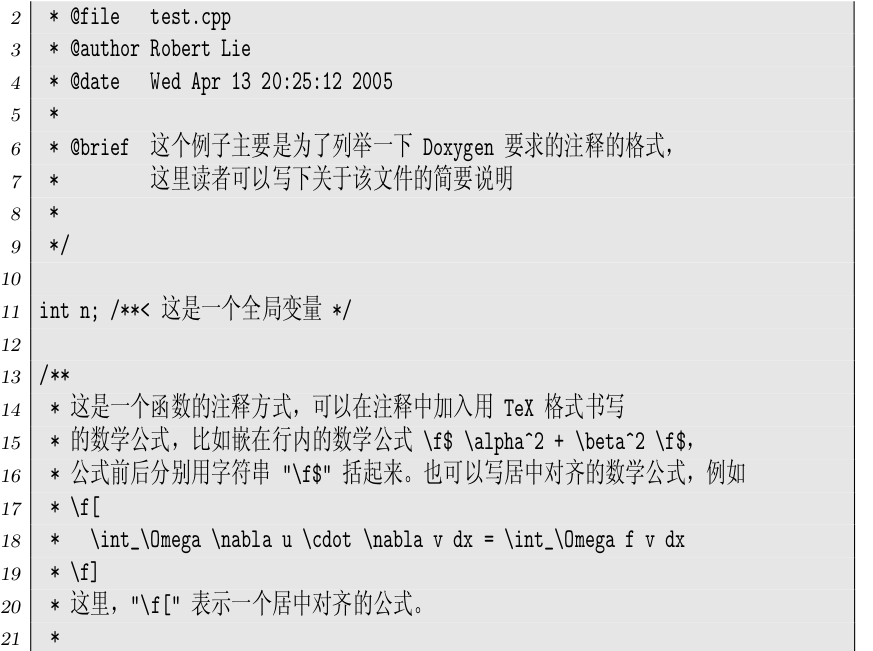
\includegraphics[scale=0.5]{./figures/14.png}
\caption{}
\end{figure}

\begin{figure}[H]
\centering
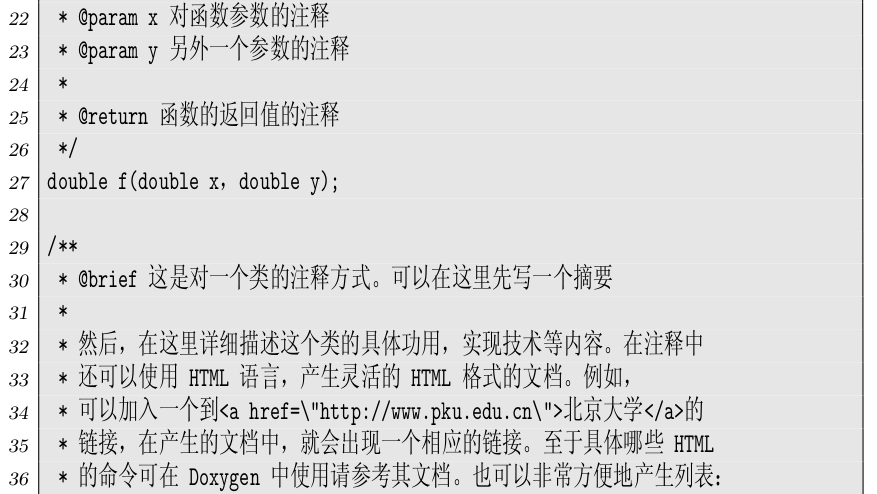
\includegraphics[scale=0.5]{./figures/15.png}
\caption{}
\end{figure}

\begin{figure}[H]
\centering
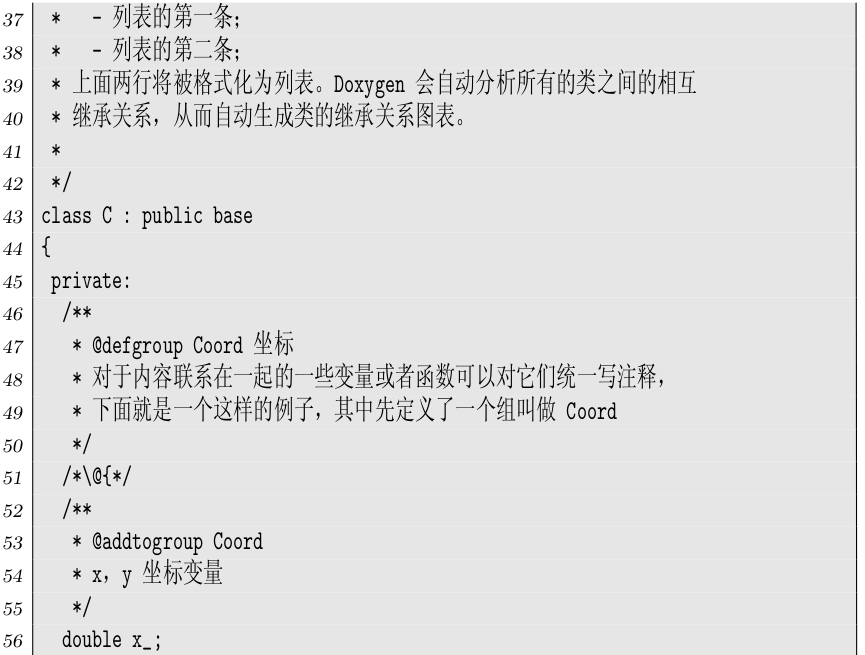
\includegraphics[scale=0.5]{./figures/16.png}
\caption{}
\end{figure}

\begin{figure}[H]
\centering
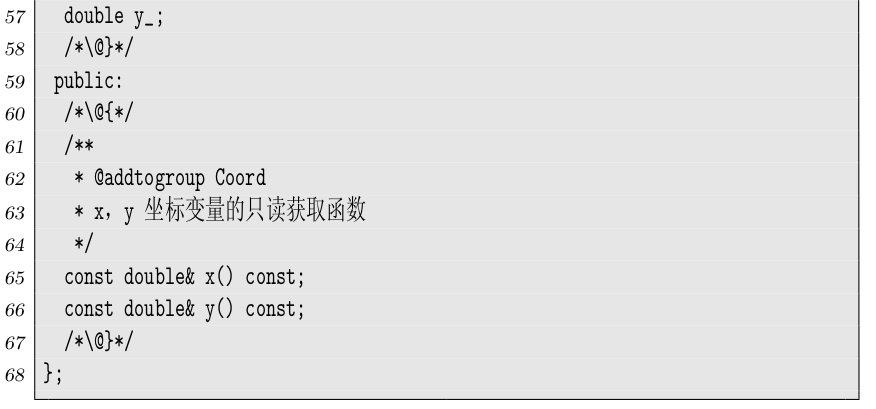
\includegraphics[scale=0.5]{./figures/17.png}
\caption{}
\end{figure}
下面准备 Doxygen 需要的配置文件。在命令行运行
\begin{figure}[H]
\centering
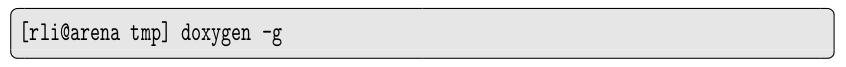
\includegraphics[scale=0.5]{./figures/18.png}
\caption{}
\end{figure}
Doxygen 会自动产生一个配置文件的模板,文件名为 Doxyfile 
\begin{figure}[H]
\centering
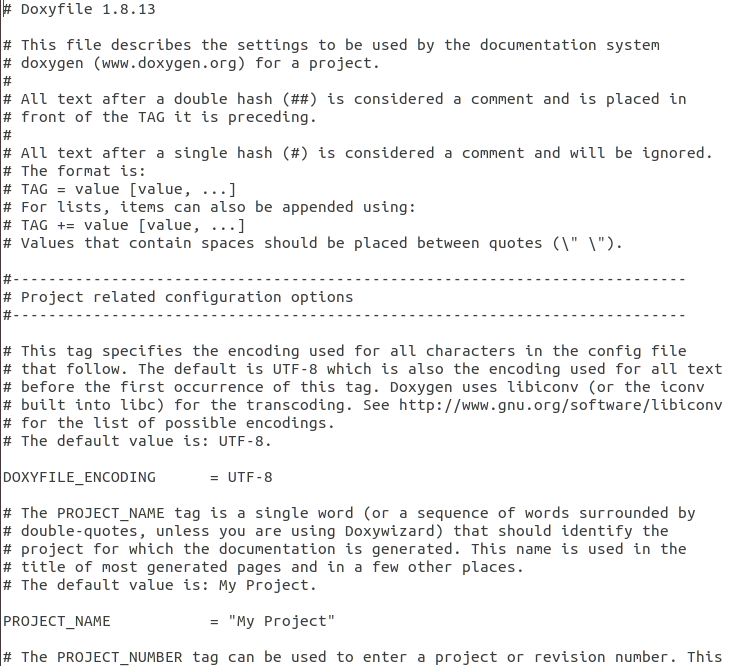
\includegraphics[scale=0.5]{./figures/33.png}
\caption{}
\end{figure}

\begin{figure}[H]
\centering
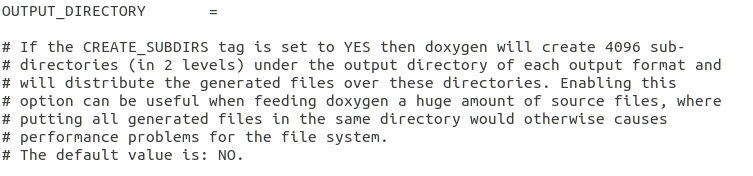
\includegraphics[scale=0.5]{./figures/34.png}
\caption{}
\end{figure}

\begin{figure}[H]
\centering
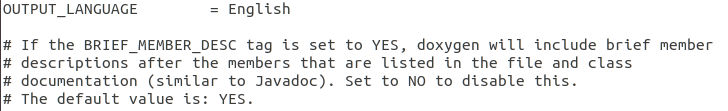
\includegraphics[scale=0.5]{./figures/35.png}
\caption{}
\end{figure}

\begin{figure}[H]
\centering
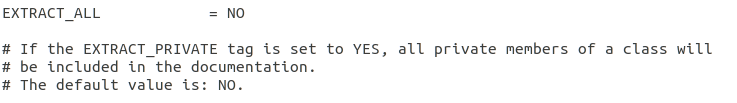
\includegraphics[scale=0.5]{./figures/36.png}
\caption{}
\end{figure}

\begin{figure}[H]
\centering
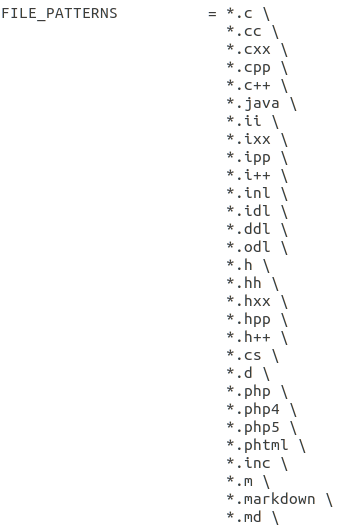
\includegraphics[scale=0.5]{./figures/37.png}
\caption{}
\end{figure}
直接编辑它便可获得所需要的配置文件。在配置文件中,通过对一些变量赋值来控制 Doxygen 的处理方式。下面列举的是配置文件中的几个主要变量。自动生成的配置文件模板中对每一个变量都进行了详细的注释,可以通过这些注释了解每个变量的意义及允许的值。
\begin{figure}[H]
\centering
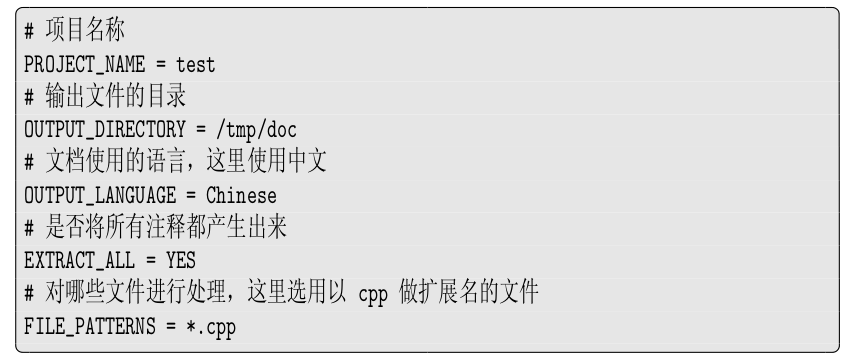
\includegraphics[scale=0.5]{./figures/19.png}
\caption{}
\end{figure}
这样 Doxygen 的配置文件就算写好了,将它放在源程序 test.cpp 所在的目录中,文件名仍然叫做 Doxyfile ,然后在目录中输入命令:
\begin{figure}[H]
\centering
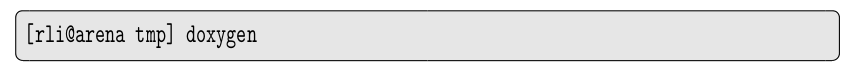
\includegraphics[scale=0.5]{./figures/20.png}
\caption{}
\end{figure}
Doxygen 便开始处理。处理过程中会显示很多信息。处理结束后,可以看到目录下多出了一个名为 doc 的目录,其中有两个子目录,分别是 latex 和 html ,存储着 L A TEX 格式的文档和 HTML 格式的文档。需要注意的是,对于中文文档的 L A TEX 文件,需要手工或是通过一个后处理脚本加入支持中文的 L A TEX 宏包,如 CCT 或 CJK ,图 2.3 是将 refman.tex 的第一行
\begin{figure}[H]
\centering
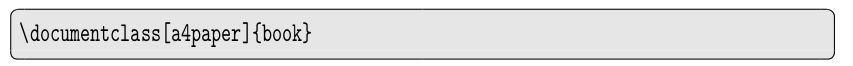
\includegraphics[scale=0.5]{./figures/21.png}
\caption{}
\end{figure}
改成
\begin{figure}[H]
\centering
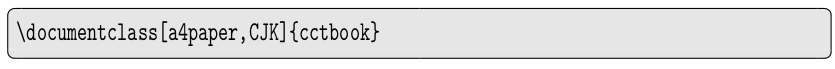
\includegraphics[scale=0.5]{./figures/22.png}
\caption{}
\end{figure}
后再用 LATEX 编译的结果。
\begin{figure}[H]
\centering
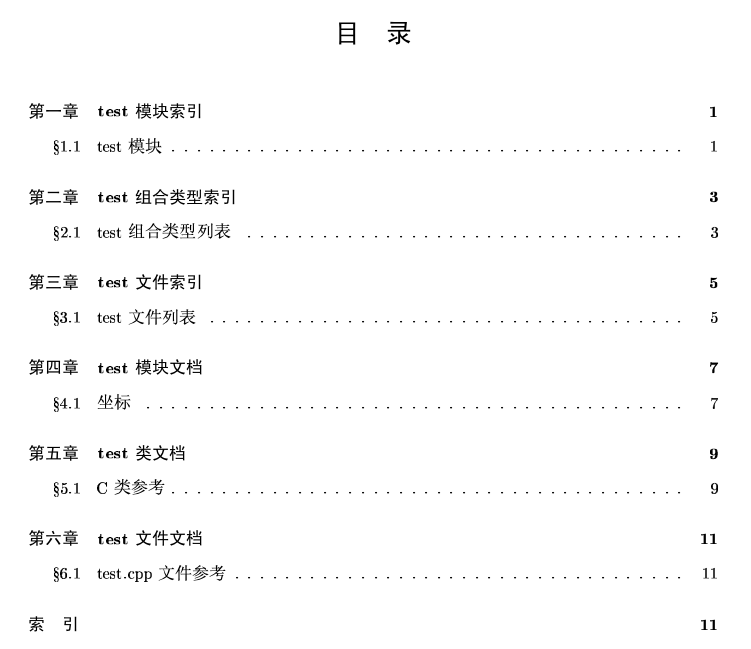
\includegraphics[scale=0.5]{./figures/23.png}
\caption{}
\end{figure}

\section{ 消息传递编程接口 MPI }
MPI (Message Passing Interface) 是一个消息传递编程标准,是为基于消息传递的并行程序设计提供一个编程环境。MPICH 是目前使用最广泛的免费 MPI 系统,本节介绍如何在 Linux 系统中安装 MPICH.

\subsection{ MPICH 的安装 }
1. 下载压缩文件,网址如下:http://www.mcs.anl.gov/mpi/mpich,从该
处可以下载mpich.tar.gz.
\begin{figure}[H]
\centering
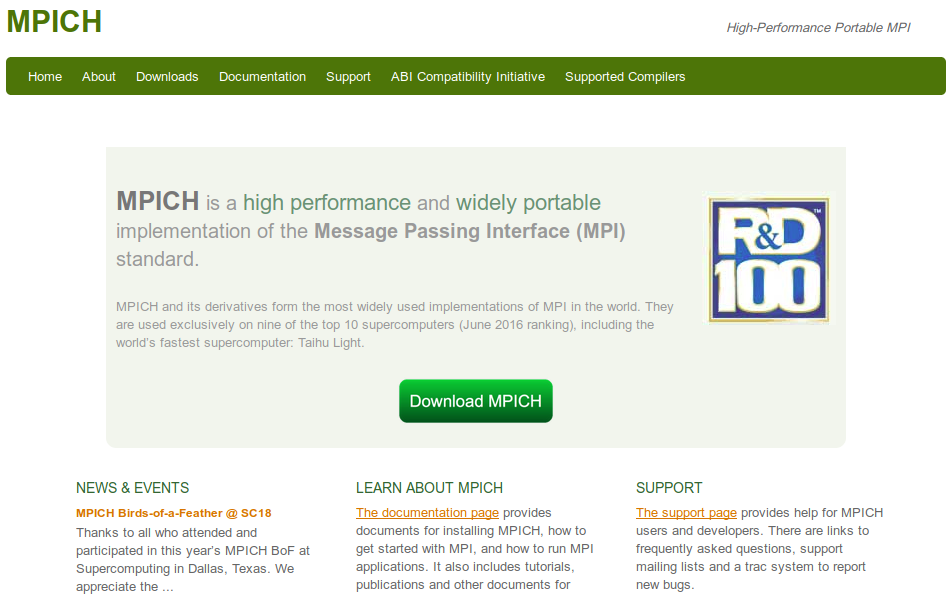
\includegraphics[scale=0.5]{./figures/1.png}
\caption{}
\end{figure}

\begin{figure}[H]
\centering
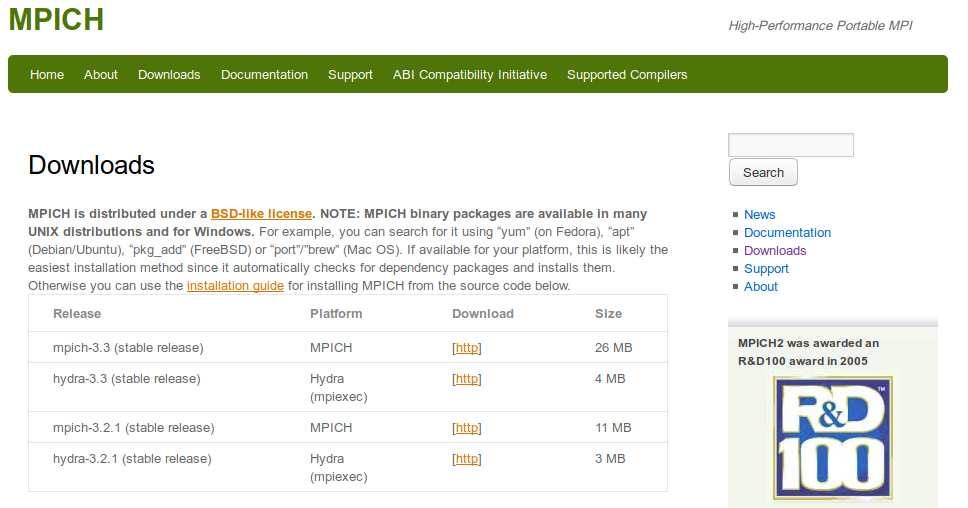
\includegraphics[scale=0.5]{./figures/2.png}
\caption{}
\end{figure}

2. 解压。下载后的解压文件在Downloads中,然后点击右键,直接解压。

3. 配置。在存放解压后的文件的环境中打开终端,输入./configure --prefix=/home/用户名/mpich-install --disable-fortran 
\begin{figure}[H]
\centering
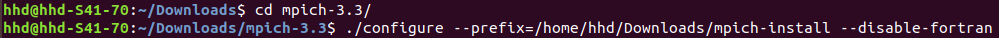
\includegraphics[scale=0.5]{./figures/3.png}
\caption{}
\end{figure}

4. make.继续输入make.
\begin{figure}[H]
\centering
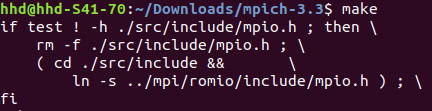
\includegraphics[scale=0.5]{./figures/4.png}
\caption{}
\end{figure}

5. make install.继续输入make install.
\begin{figure}[H]
\centering
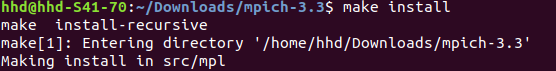
\includegraphics[scale=0.5]{./figures/5.png}
\caption{}
\end{figure}

6. 设置环境变量。在终端输入vim .bashrc,然后在vim中输入
\begin{figure}[H]
\centering
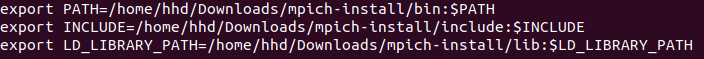
\includegraphics[scale=0.5]{./figures/38.png}
\caption{}
\end{figure}

然后再在终端输入source .bashrc
\begin{figure}[H]
\centering
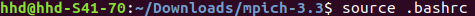
\includegraphics[scale=0.5]{./figures/7.png}
\caption{}
\end{figure}

这样MPICH就安装成功了,举例
\begin{figure}[H]
\centering
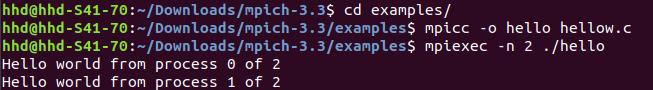
\includegraphics[scale=0.5]{./figures/8.png}
\caption{}
\end{figure}






%\bibliography{../ref}
\end{document}
